\documentclass[12pt]{beamer}
\usetheme{Warsaw}
\usepackage[utf8]{inputenc}
\usepackage{amsmath}
\usepackage{amsfonts}
\usepackage{amssymb}
\usepackage{graphicx}
\usepackage[font=Times,timeinterval=1,timeduration=2.0,timedeath=0,fillcolorwarningsecond=white!60!yellow,timewarningfirst=50,timewarningsecond=80,resetatpages=2]{tdclock}
\usepackage{tabularx}
\usepackage{array}
\usepackage{multicol}
\usepackage{longtable}
\usepackage{xcolor}
\usepackage{textcomp, gensymb}
\usepackage{pgfplots}
\usepackage[makeroom]{cancel}

\graphicspath{ {./references/} }
\pgfplotsset{
	soldot/.style={color=black,only marks,mark=*},
	holdot/.style={color=black,fill=white,only marks,mark=*},
	compat=1.12
}
\newcolumntype{Y}{>{\centering\arraybackslash}X}
\makeatletter
\def\@listii{\leftmargin\leftmarginii
			  \topsep    2ex
			  \parsep    0\p@   \@plus\p@
			  \itemsep   \parsep}
\makeatother
\newcommand\at[2]{\left.#1\right|_{#2}}

\begin{document}
\begin{frame}
	\frametitle{Bellwork 12/13}
	\initclock

	\large
	Find the area under the piecewise curve below:
	\vfill
	\begin{center}
		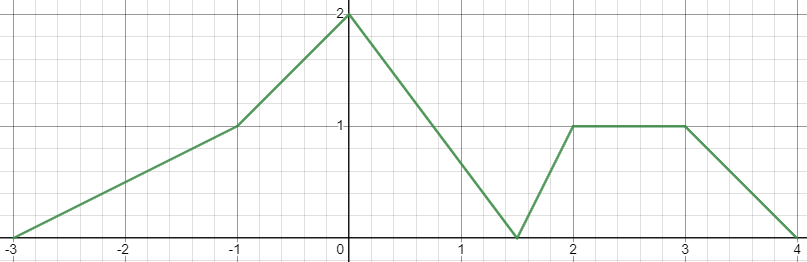
\includegraphics[scale=0.5]{bellwork_graph.png}
	\end{center}
	\vfill

	\small
	\crono
	\resetcrono{\beamerbutton{reset}}
\end{frame}
\begin{frame}
	\frametitle{Bellwork 12/13 - Solution}

	\large
	\begin{center}
		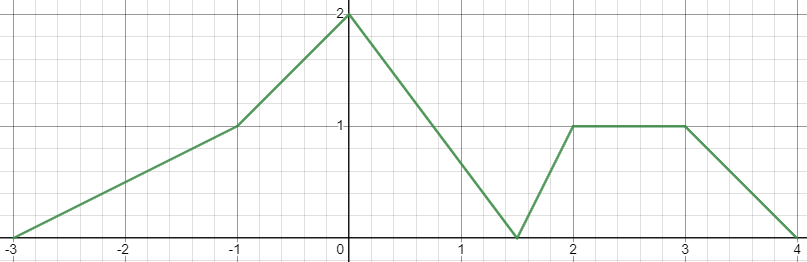
\includegraphics[scale=0.5]{bellwork_graph.png} % *: The regional areas are to be written-in on the regions.
	\end{center}
	\vfill
	\[1+\frac{3}{2}+\frac{3}{2}+\frac{9}{4}=\boxed{\frac{25}{4}}\]
\end{frame}
\end{document}